
% VLDB template version of 2020-08-03 enhances the ACM template, version 1.7.0:
% https://www.acm.org/publications/proceedings-template
% The ACM Latex guide provides further information about the ACM template

\documentclass[sigconf, nonacm, spanish]{acmart}

%% The following content must be adapted for the final version
% paper-specific
\newcommand\vldbdoi{XX.XX/XXX.XX}
\newcommand\vldbpages{XXX-XXX}
% issue-specific
\newcommand\vldbvolume{14}
\newcommand\vldbissue{1}
\newcommand\vldbyear{2021}
% should be fine as it is
\newcommand\vldbauthors{\authors}
\newcommand\vldbtitle{\shorttitle} 
% leave empty if no availability url should be set
\newcommand\vldbavailabilityurl{https://github.com/ElenaVillano/sentiment_analysis_tweets}
% whether page numbers should be shown or not, use 'plain' for review versions, 'empty' for camera ready
\newcommand\vldbpagestyle{plain} 


\usepackage[spanish]{babel}
%\patchcmd{\thebibliography}{\chapter*}{\section*}{}{} % Para que la bibliografía aparezca en la misma página
\addto\captionsspanish{\renewcommand{\bibname}{Referencias}}


\begin{document}
\title{Análisis de sentimientos con tweets}

%%
%% The "author" command and its associated commands are used to define the authors and their affiliations.
\author{Elena Villalobos}
\affiliation{%
  \institution{Instituto Tecnológico Autónomo de México}
  \city{CDMX}
}
\email{villaele14@gmail.com}

\author{Carolina Acosta}
\orcid{0000-0002-1825-0097}
\affiliation{%
  \institution{Instituto Tecnológico Autónomo de México}
  \city{CDMX}
}
\email{carolina.acostatovany@gmail.com}

\author{Edgar Bazo}
\orcid{0000-0001-5109-3700}
\affiliation{%
  \institution{Instituto Tecnológico Autónomo de México}
  \city{CDMX}
}
\email{ing.edbaz@gmail.com}


%%
%% The abstract is a short summary of the work to be presented in the
%% article.
\begin{abstract}

[Consta de un sólo párrafo.
Resumen de lo que contiene lo que estamos a punto de leer.
Dar idea de lo que podemos esperar.
Invitar al lector a leer todo el documento].
\end{abstract}

\maketitle

%%% do not modify the following VLDB block %%
%%% VLDB block start %%%
\pagestyle{\vldbpagestyle}
\begingroup\small\noindent\raggedright\textbf{PVLDB Reference Format:}\\
\vldbauthors. \vldbtitle. PVLDB, \vldbvolume(\vldbissue): \vldbpages, \vldbyear.\\
\href{https://doi.org/\vldbdoi}{doi:\vldbdoi}
\endgroup
\begingroup
\renewcommand\thefootnote{}\footnote{\noindent
This work is licensed under the Creative Commons BY-NC-ND 4.0 International License. Visit \url{https://creativecommons.org/licenses/by-nc-nd/4.0/} to view a copy of this license. For any use beyond those covered by this license, obtain permission by emailing \href{mailto:info@vldb.org}{info@vldb.org}. Copyright is held by the owner/author(s). Publication rights licensed to the VLDB Endowment. \\
\raggedright Proceedings of the VLDB Endowment, Vol. \vldbvolume, No. \vldbissue\ %
ISSN 2150-8097. \\
\href{https://doi.org/\vldbdoi}{doi:\vldbdoi} \\
}\addtocounter{footnote}{-1}\endgroup
%%% VLDB block end %%%

%%% do not modify the following VLDB block %%
%%% VLDB block start %%%
\ifdefempty{\vldbavailabilityurl}{}{
\vspace{.3cm}
\begingroup\small\noindent\raggedright\textbf{PVLDB Artifact Availability:}\\
El código fuente, notebooks y otros recursos estan disponibles en: \url{\vldbavailabilityurl}.
\endgroup
}
%%% VLDB block end %%%

\section{Introducción}


%Un párrafo explicando el problema que vamos a enfrentar.
Hoy en día, las redes sociales son un medio de comunicación muy utilizado para conocer las opiniones actuales sobre diversos temas. Una primera aproximación para conocer y/o describir los procesos de comunicación en estas redes, es saber si los comentarios u opiniones tienen alguna connotación positiva o negativa. Una de las redes sociales más utilizadas para monitorear la conversación pública es Twitter; por lo que, en el nos enfocaremos a estudiar dicha red social. Específicamente, el objetivo del presente proyecto es analizar el contenido de tweets y poder construir un clasificador que aprenda a distinguir entre una opinión positiva o negativa.

%Uno o dos párrafos(puede ser subsección) explicando los datos(fuente, tamaño de la bd, no. de variables, formato de entrada x y salida y, hay outliers? , divisón entrenamiento, validación y prueba.

Los datos que utilizaremos fueron recolectados de Twitter, por la empresa H20 \cite{H20}, acerca del Huracán Harvey y tweets con intención negativa o seria. El conjunto de datos tiene las siguientes características:

\begin{itemize}
\item Idioma: Inglés.
\item Observaciones: 1.6 millones.
\item Variables: 
    \begin{itemize}
    \item \texttt{target:} Polaridad del tweet, positivo o negativo. 
    \item \texttt{ids:} ID tweet.
    \item \texttt{date:} Fecha y hora del tweet.
    \item \texttt{flag:} Si hubo algún tipo de QUERY.
    \item \texttt{user:} Usuario del tweet
    \item \texttt{text:} Texto del tweet
    \end{itemize}
\end{itemize}

La variable que utilizaremos para entrenar es \texttt{text}, que contiene sólo el tweet sin emojis; y la variable que utilizaremos como etiqueta es la \texttt{target}, que contiene el 50\% de observaciones positivas y 50\% negativas, es decir, esta balanceada.

%Mencionar brevemente qué tipo de modelo usan para atacar el problema
En este proyecto construiremos un modelo con base en Procesamiento de Lenguaje Natural (NLP por sus siglas en inglés) para realizar el análisis de sentimientos. El Procesamiento del Lenguaje Natural es el campo de estudio que se enfoca en la compresión del lenguaje humano mediante una computadora, siendo así una rama de aprendizaje profundo.

\section{Trabajos relacionados}

%Comentar brevemente algunos trabajos que puedan leer, y que hayan hecho algo similar, al menos 3 trabajos. 

%Un párrafo por trabajo, qué datos usaron, y qué problemas partirucalres reportan, qué modelo usaron, cómo es la calidad de su solución.

Jacob, en StreamHacker\cite{Jacob}, describe que se enfocó en la clasificación de sentimientos positivos o negativos. Utilizó datos del paquete NLTK para el corpus de reviews de películas. Empezó utilizando un simple clasificador de Naive Bayes como base, y extrajo las variables de forma booleana. Con poca manipulación de los datos logró obtener una exactitud del 73\%, lo cual es cerca de la exactitud humana; se dice que los humanos concuerdan en sentimientos sólo el 80\% del tiempo.

El objetivo del proyecto que realizó Laurent Luce\cite{Laurent} es clasificar un tweet positivo o negativo. Utilizó datos que extrajo manualmente, y fueron alrededor de 600 tweets positivos y 600 tweets negativos para el entrenamiento del clasificador. Utilizó tweets sin hashtags, sin menciones ni emojis. La única imputación que realizó fue eliminar las palabras menores de 2 letras y tener todo en minúsculas. Para crear el clasificador, primero se hizo una extracción de variables para saber cuáles eran las variables relevantes; y el clasificador utilizado fue Naives Bayes de NLTK. Con sus datos de prueba logró un 80\% de exactitud.

La empresa que desarrolla H20\cite{H20}, realizó un proyecto donde el objetivo fue extraer tweets relevantes para el caso del huracán Harvey, utilizando el dataset de 'sentiment140' que ya estan etiquetados como sentimientos positivos o negativos, y así construir un clasificador que aprenda a diferenciar entre un tweet negativo o serio y un tweet positivo; posterioremente el siguiente objetivo fue utilizar este clasificador para rankear los tweets basados en un porcentaje de severidad y así poder extraer el top de tweets que necesiten ayuda en la situación actual, en este caso, el huracán Harvey o Irma. Para la transformación de sus datos utilizaron TF-IDF, éste extrae para cada palabra qué tan importante es para ese tweet. Después de la transformación, utilizaron H20 Gradient Boosting para entrenar y obtener el clasificador que diferencíe entre un tweet positivo o negativo. No indican cuál es el porcentaje de su exactitud obtenida.

\section{Análisis exploratorio}



\section{Solución}

\subsection{Limpieza de datos}
%Primero explicar cualquier preprocesamiento que hayan hecho sobre los datos. 
Antes de realizar cualquier tarea de Procesamiento de Lenguaje Natural es importante que nuestros datos tengan cierto grado de limpieza. En la \autoref{tab:commands} mostramos ejemplos de textos procesados por nuestro algoritmo que contiene las siguientes tareas de limpieza:

\begin{enumerate}
\item Convertir todo el texto a minúsculas
\item Quitar:
\begin{enumerate}
    \item Caracteres codificados en html (\&amp;, \&quot;, \&lt;, \&gt;)
    \item URLs, menciones a usuarios y RT
    \item \# y mantener sólo la palabra o conjunto de palabras
    \item Espacios o puntos extras
    \item Caracteres especiales (’"?!,.():;-)
    \item Letras repetidas (sooooo haaappy)
    \item Caracteres ascii y Descifrar a utf-8
\end{enumerate}
\item Separar abreviaciones
\item Quitar stopwords
\item Realizar stemming y lematización
\item Modificar etiquetas (0 = negativo, 1 = positivo)

\end{enumerate}


\begin{table*}[t]
  \caption{Ejemplo de limpieza de texto}
  \label{tab:commands}
  \begin{tabular}{|c|c|}
    \toprule
    Texto original & Texto limpio \\
    \midrule
    \vtop{\hbox{\strut @switchfoot http://twitpic.com/2y1zl - awww, that's a bummer.}\hbox{\strut you shoulda got david carr of third day to do it. ;d }}
    & aww bummer shoulda got david carr third day  \\
    \hline
    @RunningGolfer Glad you picked it up...she didn't &  lad pick upsh   \\
    \hline
    @i140 I'm excited I made it on your list.  Thnx, Jason. &  excit made list thnx jason   \\
    \hline
    \vtop{\hbox{\strut @johncmayer Where is that Belgian concert you were}\hbox{\strut talking about? I can't even find it on google  }}
    & belgian concert talk even find googl  \\
    \hline
    \vtop{\hbox{\strut sitting on a field with Emma and Miri watching Sarah and }\hbox{\strut Naomi running around searchinf for elves }}
    & 
    \vtop{\hbox{\strut sit field emma miri watch sarah  }\hbox{\strut naomi run around searchinf elv  }}  \\
    \hline
    \vtop{\hbox{\strut Couldn't decide if I wanted to go to Family Fortunes on Sunday  }\hbox{\strut but train is  £45 now   Its the Christmas special being filmed on that day!! }}
    & 
    \vtop{\hbox{\strut could decid want go famili fortun sunday  }\hbox{\strut train 45 christma special film day  }}  \\
    
    \bottomrule
  \end{tabular}
\end{table*}

Para quitar texto o ciertos caracteres de nuestro texto, utilizamos expresiones regulares, que a continuación presentamos cada una de ellas.

\subsubsection{Caracteres HTML}

En los tweets encontramos caracteres con código HTML que se utilizan con frecuencia, como: \&, ", < y >. Cada uno tiene su código en HTML representado por: "\&amp;", "\&quot;", "\&lt"; y "\&gt"; respectivamente. Y su expresión regular es exactamente el código representado.

\subsubsection{URLs}

Las Uniform Resource Locator, (URL por sus siglas en inglés), son utilizadas en los tweets de manera frecuente para indicar la liga a una página web. La expresión regular que corresponde es \textt{((www\backslash.[\backslash S]+)|(https?://[\backslash S]+))}.

\subsubsection{Menciones a usuarios}

Es común que los usuarios mencionen a otros usuarios, y ésto se realiza con el caracter @. La expresión regular asociada a identificar las menciones es \textt{@[\backslash S]+}.

\subsubsection{Retweets}

Los Retweets son publicaciones duplicadas desde otro usuario y para identificarlas con expresiones regulares utilizamos \textt{\backslash brt\backslash b}.

\subsubsection{Hasthags}

El procesamiento de los hashtags, es simplemente eliminar el caracter \# y quedarnos con la palabra. Para identificar un hasthag con expresiones regulares utilizamos \textt{#(\backslash S)+}.

\subsubsection{Letras repetidas}

Es común que los usuarios expresen sus sentimientos repitiendo letras como "I'm sooooo haaaapppyyyy", lo cual es variable entre usuarios y decidimos reducir la repetición a lo máx 2 letras repetidas por letra, ya que en el idioma inglés es común tener letras repetidas en las palabras como "happy". De igual forma utilizamos expresiones regulares para identificar estos casos y su correspondiente es \textt{(.)\backslash 1+', r'\backslash 1\backslash 1}.

Describimos a continuación otras tareas de limpieza que decidimos mantener en nuestro proceso.

\subsubsection{Stopwords}

Para nuestra limpieza también decidimos remover las stopwords, que son palabras que realmente no aportan mucho sentido a una oración. Éstas las obtuvimos de la paquetería NLTK utilizando el idioma inglés.

\subsubsection{Stemming y lematización}

Se refiere a eliminar sufijos morfológicos a una palabra; es decir, reducir la palabra a un 'lema'; por ejemplo, "mention", "mentioning", "mentioned" son palabras que su lema llega a ser "ment". Para realizar este proceso utilizamos la paquetería de NLTK, el tokenizador word\_tokenizer y el stem "PorterStemmer". 

\subsubsection{Modificación de etiquetas}

Los datos originales contiene una variable "target" que tomamos como etiqueta, y los valores que puede tomar son "0" o "4" si son negativos o positivos respectivamente. Para nuestro problema decidimos cambiarlo a "0" y "1" para negativos y positivos respectivamente; ya que la distancia entre 0 y 1 es más corta que 0 y 4 para un clasificador.

\subsection{Tokenizador}
%Explicar su mejor modelo.
Posteriormente a la limpieza de texto, nos enfocamos en hacer otro tipo de preprocesamiento al texto utilizando un Tokenizador, que se encarga de vectorizar el texto; es decir, convierte cada palabra en una secuencia de enteros. Nosotros utilizamos el Tokenizador de Tensorflow (tensorflow.keras.preprocessing.text), y decidimos que nuestro vocabulario será de tamaño 1,000; ya que exploramos la frecuencia de cada palabra y a pesar de tener más de 50 mil palabras, no existía alta frecuencia, nos quedamos con las palabras que tenían una frecuencia arriba de 1,000.

Después de obtener el tokenizador con nuestro vocabulario, identificamos que nuestro máximo de palabras por oración es XX palabras, por lo que tuvimos que realizar un padding; es decir transformar cada secuencia de tokens al mismo tamaño. Utilizamos el post padding, que agrega el pad(0) después de cada secuencia. De igual forma utilizamos Tensorflow (tensorflow.keras.preprocessing. sequence).

\subsection{Arquitectura de la red neuronal}

Nuestro modelo es secuencial...

Para explicar mejor la arquitectura de nuestra red neuronal,  hemos extraído la \autoref{fig:architecture}. Y en breve explicaremos cada una de las capas contenidas en nuestro modelo.
.


\begin{figure}
  \centering
  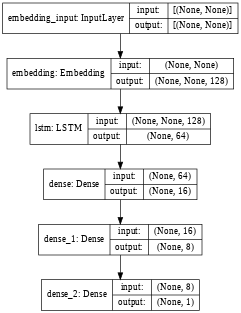
\includegraphics[width=\linewidth]{figures/arquitectura}
  \caption{Extracción del diagrama de nuestro modelo en \textit{Tensorflow.Keras}}
  \label{fig:architecture}
\end{figure}

\subsubsection{Embedding} 

La capa de Embeddings se utiliza al principio de la red neuronal, ya que ésta es la encargada de realizar el procesamiento de texto. Como parámetros de especificamos el tamaño del vocabulario, la dimensión de nuestra salida y la longitud de las secuencias, que en nuestro caso como habíamos mencionado anteriormente es XX.

\subsubsection{Long Short Term Memory}

LSTM por sus siglas en inglés. Que hace referencia a una red neuronal recurrente de memoria a corto plazo. Buscamos una red neuronal recurrente porque existe retroalimentación entre neuronas y es lo que se necesita para realizar procesamiento de lenguaje natural. Es común que en entradas de datos suficientemente grandes la red no sea capaz de conectar dependencias y por lo mismo se pierde la cohesión; las redes LSTM solucionan este problema.

Una vez definidas las capas que utilizaremos, configuramos el modelo para utilizar:

\begin{itemize}
    \item Optimizador
    
    RMSProp
    
    \item Función de pérdida
    
    Binary Cross Entropy.
    
    \item Métricas
    
    Binary accuracy y accuracy.
    
\end{itemize}

Para entrenar utilizamos XXX datos de los cuales 20\% utilizamos para validación.

Utilizamos 10 épocas y un tamaño de batch de 64.

\subsection{Comparaciones}
%Mencionar otras opciones que hayamos probado. 

Experimentamos con varios modelos para poder extraer el que mejor se comportaba, algunos de los parámetros que cambiamos fueron los siguientes:

\begin{itemize}
    \item Función de costo
\end{itemize}

Explicarlas en función de sus diferencias al mejor modelo (tablas comparativas puede ayudar)


\subsection{Math and Equations}

Curabitur vitae nulla dapibus, ornare dolor in, efficitur enim. Cras fermentum facilisis elit vitae egestas. Nam vulputate est non tellus efficitur pharetra. Vestibulum ligula est, varius in suscipit vel, porttitor id massa. Cras facilisis suscipit orci, ac tincidunt erat.
\begin{equation}
  \lim_{n\rightarrow \infty}x=0
\end{equation}

Sed pulvinar lobortis dictum. Aliquam dapibus a velit porttitor ultrices. Ut maximus mi id arcu ultricies feugiat. Phasellus facilisis purus ac ipsum varius bibendum. Aenean a quam at massa efficitur tincidunt facilisis sit amet felis. 
\begin{displaymath}
  \sum_{i=0}^{\infty} x + 1
\end{displaymath}

Suspendisse molestie ultricies tincidunt. Praesent metus ex, tempus quis gravida nec, consequat id arcu. Donec maximus fermentum nulla quis maximus.
\begin{equation}
  \sum_{i=0}^{\infty}x_i=\int_{0}^{\pi+2} f
\end{equation}

Curabitur vitae nulla dapibus, ornare dolor in, efficitur enim. Cras fermentum facilisis elit vitae egestas. Nam vulputate est non tellus efficitur pharetra. Vestibulum ligula est, varius in suscipit vel, porttitor id massa. Cras facilisis suscipit orci, ac tincidunt erat.



\section{Resultados}

Presentar resultados obtenidos.

Curvas de desempeño, tablas, matrices de confusión, etc.

Explicar razones encontradas para el desempeño obtenido.

Discutir resultados.

Mencionar problemas encontrados, tanto solucionados como los que no se hayan podido superar.

\section{Conclusiones}

Presentar conclusiones.

Qué se logró.

Qué obstáculos quedan por superar. Cómo sugieren hacerlo.

Qué problemas enfrentaron.

Qué aprendimos.

%\begin{acks}
% This work was supported by the [...] Research Fund of [...] (Number [...]). Additional funding was provided by [...] and [...]. We also thank [...] for contributing [...].
%\end{acks}

%\clearpage

\begin{thebibliography}{4}

\bibitem{H20}
\textit{Social Machine Learning with H20, Twitter, python}. Última consulta: 25/05/2019
\url{https://www.linkedin.com/pulse/social-machine-learning-h2o-twitter-python-marios-michailidis/}

\bibitem{Jacob}
\textit{Jacob, 2010. StreamHacker. Text classification for sentiment analysis - Naive Bayes Classifier}
\url{https://streamhacker.com/2010/05/10/text-classification-sentiment-analysis-naive-bayes-classifier/}

\bibitem{Laurent}
\textit{Laurent Luce, 2012. LaurentLuce. Twitter sentiment analysis using Python and NLTK}
\url{http://www.laurentluce.com/posts/twitter-sentiment-analysis-using-python-and-nltk/}

\bibitem{Klein} %Para libros
Klein, J. P. \& Moeschberger.
\textit{Survival Analysis}.
Springer, 1997. 

\end{thebibliography}
\end{document}
\endinput
